\documentclass[11pt]{article}
\usepackage{geometry}                % See geometry.pdf to learn the layout options. There are lots.
\geometry{letterpaper}                   % ... or a4paper or a5paper or ... 
%\geometry{landscape}                % Activate for for rotated page geometry
%\usepackage[parfill]{parskip}    % Activate to begin paragraphs with an empty line rather than an indent
\usepackage{graphicx}
\usepackage{amssymb}
\usepackage{amsmath}
\usepackage{epstopdf}
\usepackage{hyperref}
\DeclareGraphicsRule{.tif}{png}{.png}{`convert #1 `dirname #1`/`basename #1 .tif`.png}


\graphicspath{
{/Users/Andy/Cruises_Research/Analysis/Andy_Pickering/micro_database/figures/}
}

\title{Analysis of some data from microstructure database}
\author{Andy Pickering}
%\date{}                                           % Activate to display a given date or no date



\begin{document}
\maketitle

\tableofcontents
\newpage



%~~~~~~~~~~~~~~~~~~~~~~~~~~~~~~~~~~~~~~~~~~~~~~~~~~
\section{Overview}
%~~~~~~~~~~~~~~~~~~~~~~~~~~~~~~~~~~~~~~~~~~~~~~~~~~


Analysis of some global microstructure datasets, to compare the results to my EQ14 analysis. Specifically I am looking at $\gamma$ and the ratio of $\epsilon_{\chi}/\epsilon$, where $\gamma$ is the mixing efficiency ( more accurately mixing coefficient?) and $\epsilon_{\chi}$ is computed as 

\begin{equation}
\epsilon_{\chi} = \frac{N^2\chi}{2\gamma T_{z}^{2}}
\end{equation}
, in the framework of trying to estime $\epsilon$ from thermistor profiles.





%~~~~~~~~~~~~~~~~~~~~~~~~~~~~~~~~~~~~~~~~~~~~~~~~~~
\section{Data}
%~~~~~~~~~~~~~~~~~~~~~~~~~~~~~~~~~~~~~~~~~~~~~~~~~~


\begin{itemize}

\item Data are from the microstructure data base at \url{https://microstructure.ucsd.edu/}. I am using matlab files made from the raw database files by Amy Waterhouse (shared w/ me via Google drive). 

\item IWISE 11 vmp data were shared with me by Lou St. Laurent.

\item EQ14 data are from Jim Moum and group at OSU.

\end{itemize}



%~~~~~~~~~~~~~~~~~~~~~~~~~~~~~~~~~~~~~~~~~~~~~~~~~~
\section{Code}
%~~~~~~~~~~~~~~~~~~~~~~~~~~~~~~~~~~~~~~~~~~~~~~~~~~

Code and results (including figures and these notes) are available in a github repository: \url{https://github.com/OceanMixingGroup/Analysis/tree/master/Andy_Pickering/micro_database}

\begin{itemize}

\item \verb+Plot_micro_data_AP.m+

\item \verb+Plot_hist_chieps_chi_all.m+

\item \verb+Plot_epschi_eps_2Dhist_all.m+

\item \verb+ Plot_chi_eps_norm_all.m+

\end{itemize}






%~~~~~~~~~~~~~~~~~~~~~~~~~~~~~~~~~~~~~~~~~~~~~~~~~~
\section{Results}
%~~~~~~~~~~~~~~~~~~~~~~~~~~~~~~~~~~~~~~~~~~~~~~~~~~




\clearpage
%~~~~~~~~~~~~
\subsection{Histograms of $\chi$ and $\epsilon$}
%~~~~~~~~~~~~

Most of the data sets contain mostly small values of $\epsilon$ (Figure \ref{chiepshists}). Graviluck and IWISE11 seem to be the only ones w/ $\epsilon$ values as large as EQ08.

\begin{figure}[htbp]
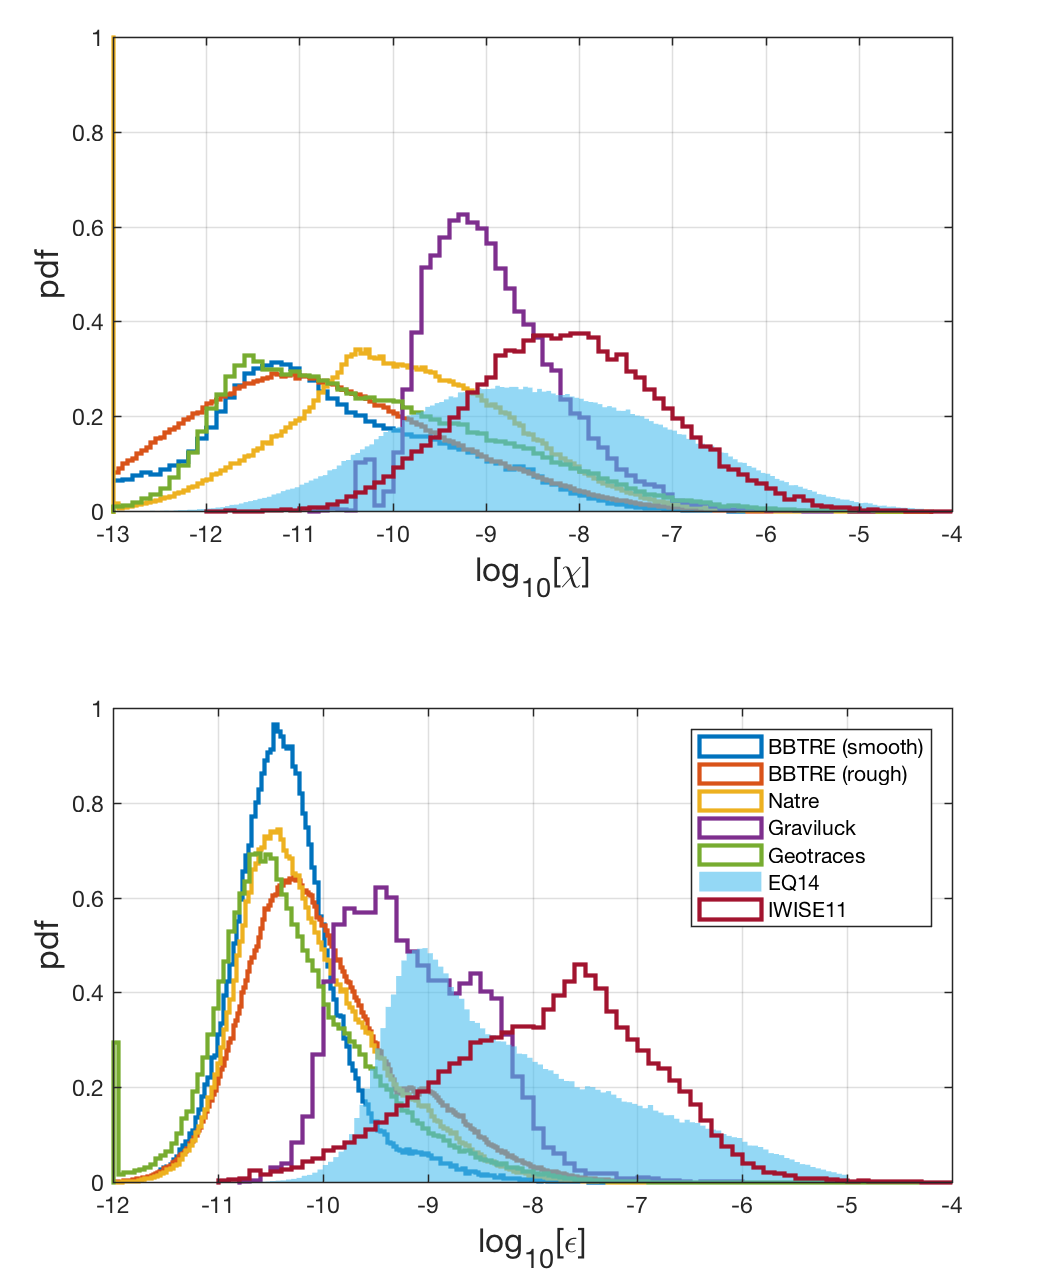
\includegraphics[scale=0.8]{eps_hist_ALL.png}
\caption{Histograms of (log10)  $\chi$ and $\epsilon$ for different data sets.}
\label{chiepshists}
\end{figure}




\clearpage
%~~~~~~~~~~~~
\subsection{2D Histograms of $\epsilon_{\chi}$ vs $\epsilon$}
%~~~~~~~~~~~~

Figures \ref{2Dhist} and \ref{2Dhistthresh} show 2D histograms of $\epsilon_{\chi}$ vs $\epsilon$ for the various data sets. Based on Figure \ref{2Dhist}, I estimated the $\epsilon$ noise level at about $log_{10}\epsilon=-10$ (except for EQ14, which is estimated to be -8.5). Data below these noise levels are exluded in Figure \ref{2Dhistthresh}.

\begin{figure}[htbp]
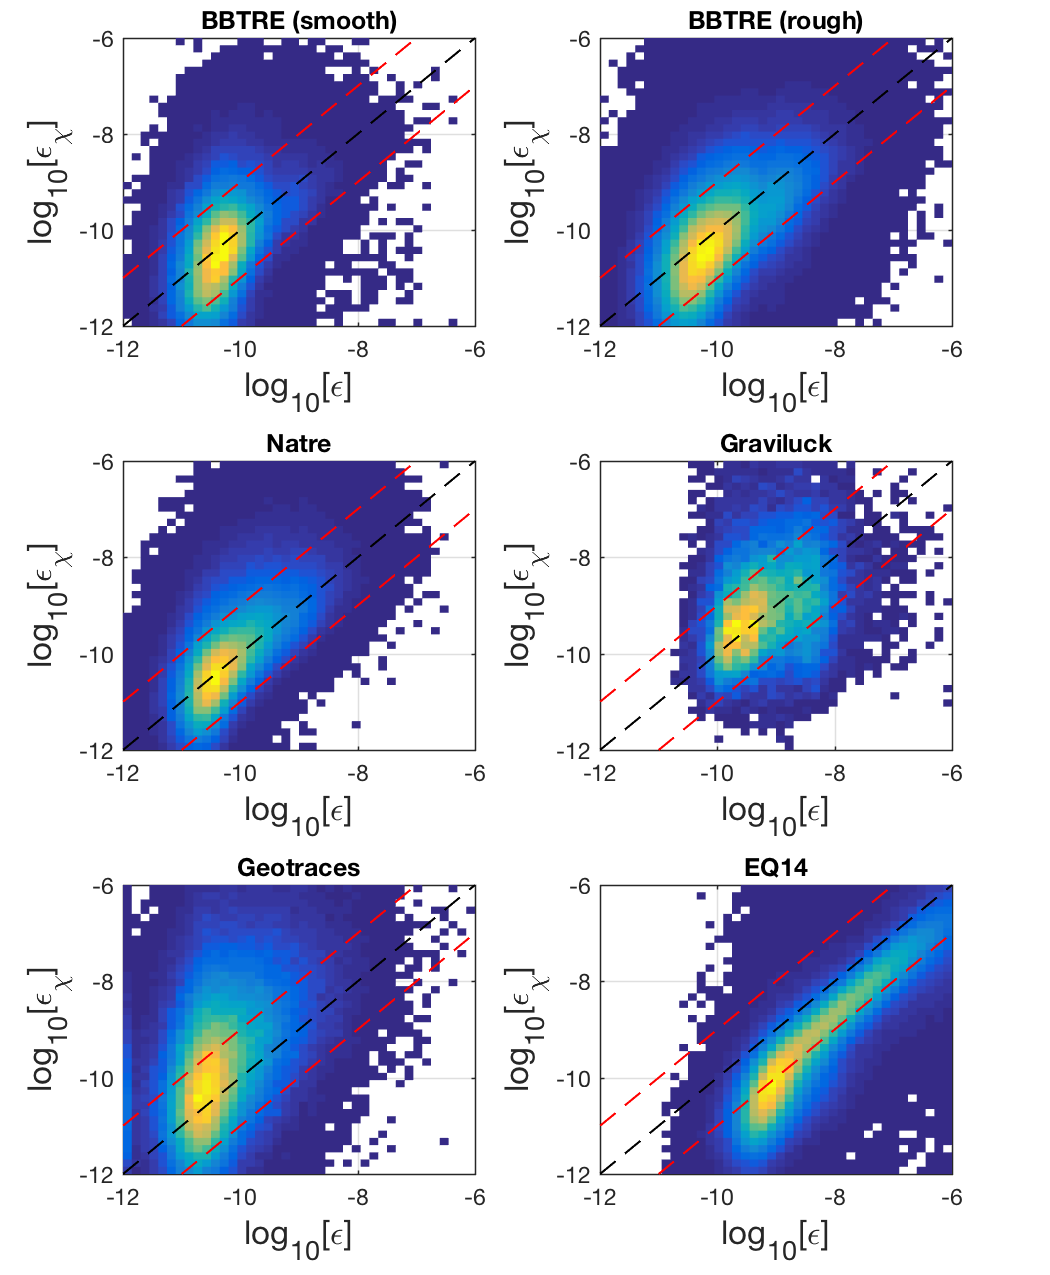
\includegraphics[scale=0.8]{epschi_eps_2Dhist_ALL.png}
\caption{2D histograms of $\epsilon_{\chi}$ vs $\epsilon$.}
\label{2Dhist}
\end{figure}


\begin{figure}[htbp]
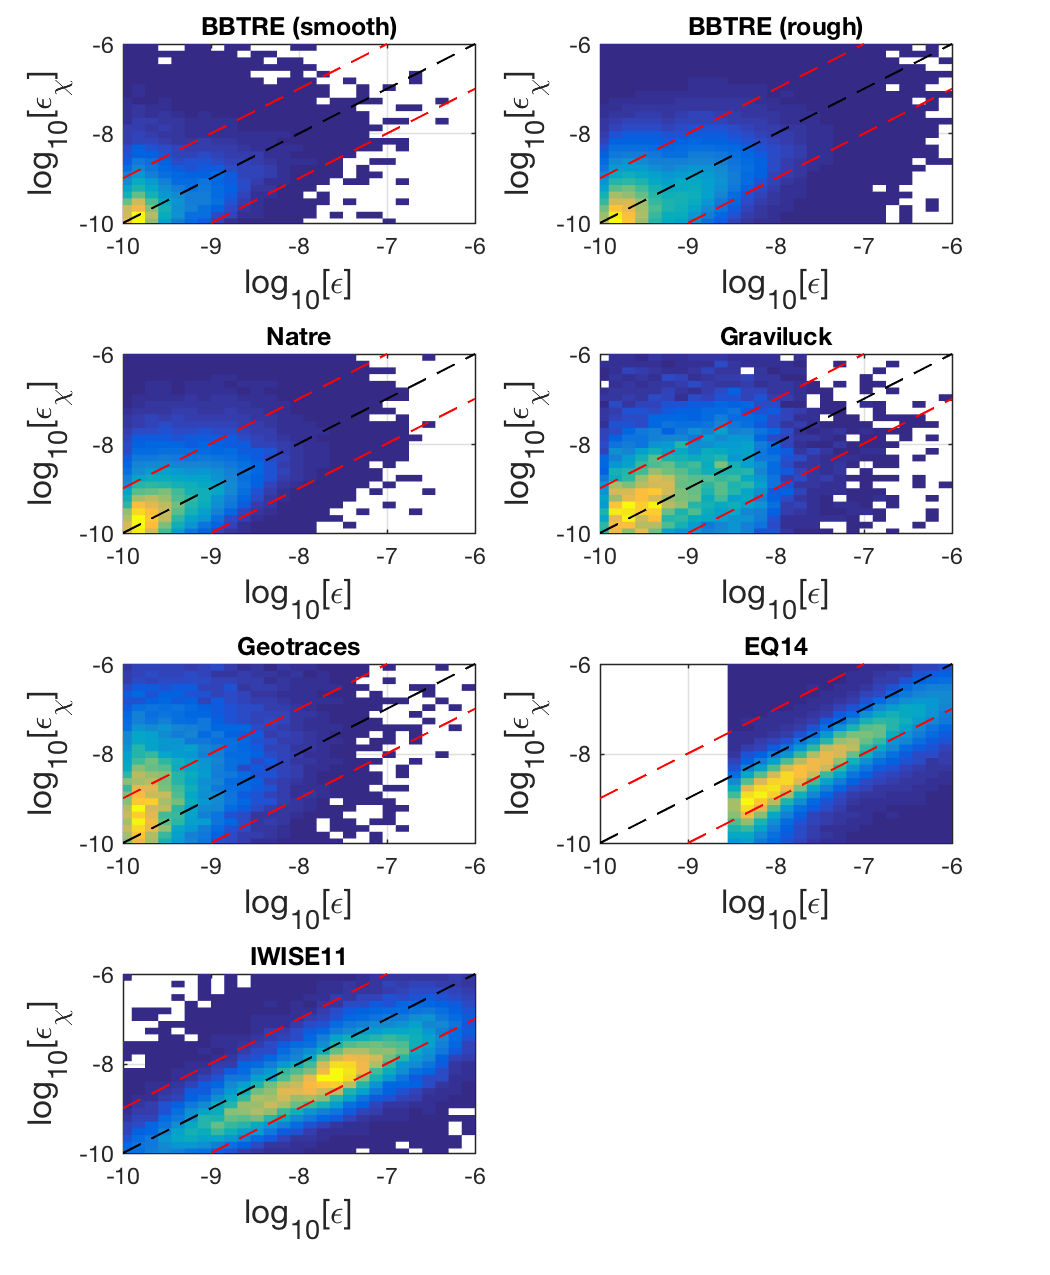
\includegraphics[scale=0.8]{epschi_eps_2Dhist_ALL_eps_thresh.png}
\caption{2D histograms of $\epsilon_{\chi}$ vs $\epsilon$. Values below estimated noise level of $log_{10}[\epsilon]=-10$ discarded.}
\label{2Dhistthresh}
\end{figure}




\clearpage
%~~~~~~~~~~~~
\subsection{Histograms of $\epsilon_{\chi}/\epsilon$}
%~~~~~~~~~~~~


\begin{itemize}

\item EQ08 and IWISE11 are biased low. Geotraces is biased high. Most of the others are close to 0.

\end{itemize}


\begin{figure}[htbp]
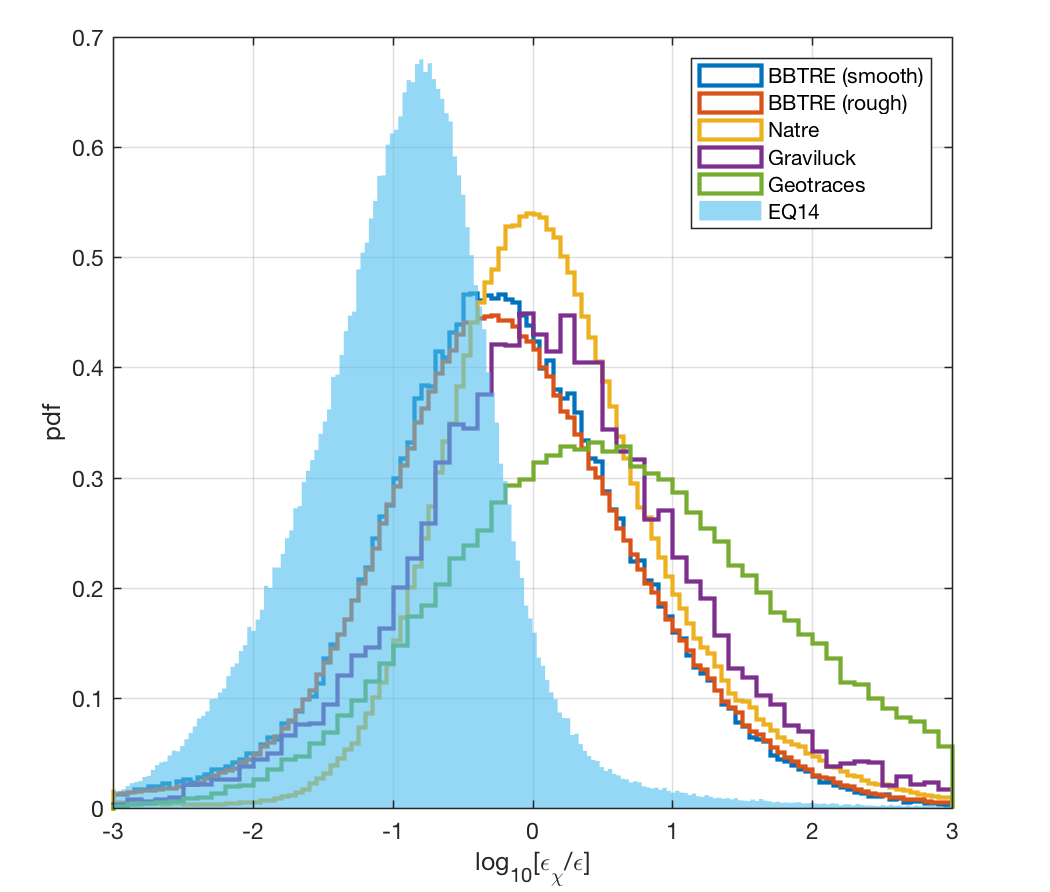
\includegraphics[scale=0.8]{epschi_eps_hist_ALL.png}
\caption{Histograms of (log10) the ratio $\epsilon_{\chi}/\epsilon$ for different data sets.}
\label{}
\end{figure}


\begin{figure}[htbp]
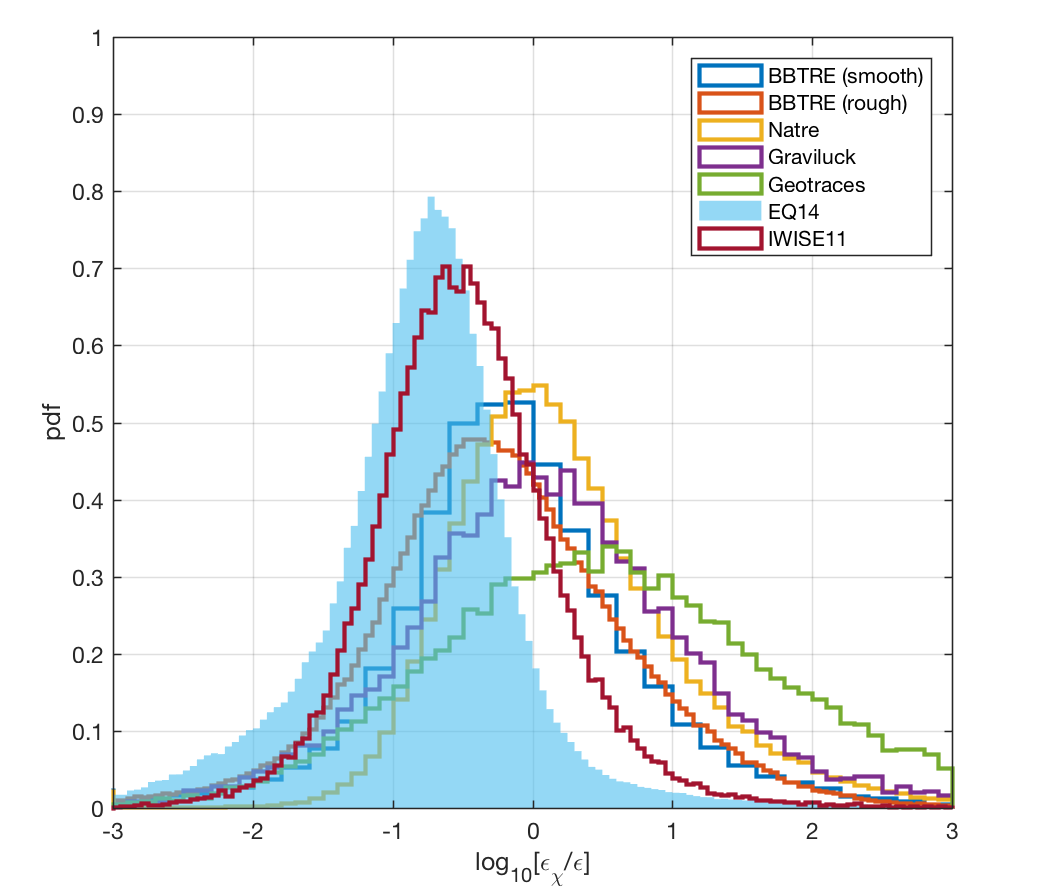
\includegraphics[scale=0.8]{epschi_eps_hist_ALL_eps_thresh.png}
\caption{Histograms of (log10) the ratio $\epsilon_{\chi}/\epsilon$. Values below estimated noise level of $log_{10}[\epsilon]=-10$ discarded.}
\label{}
\end{figure}





\clearpage
%~~~~~~~~~~~~
\subsection{Plots of normalized $\chi$ vs $\epsilon$}
%~~~~~~~~~~~~

\begin{figure}[htbp]
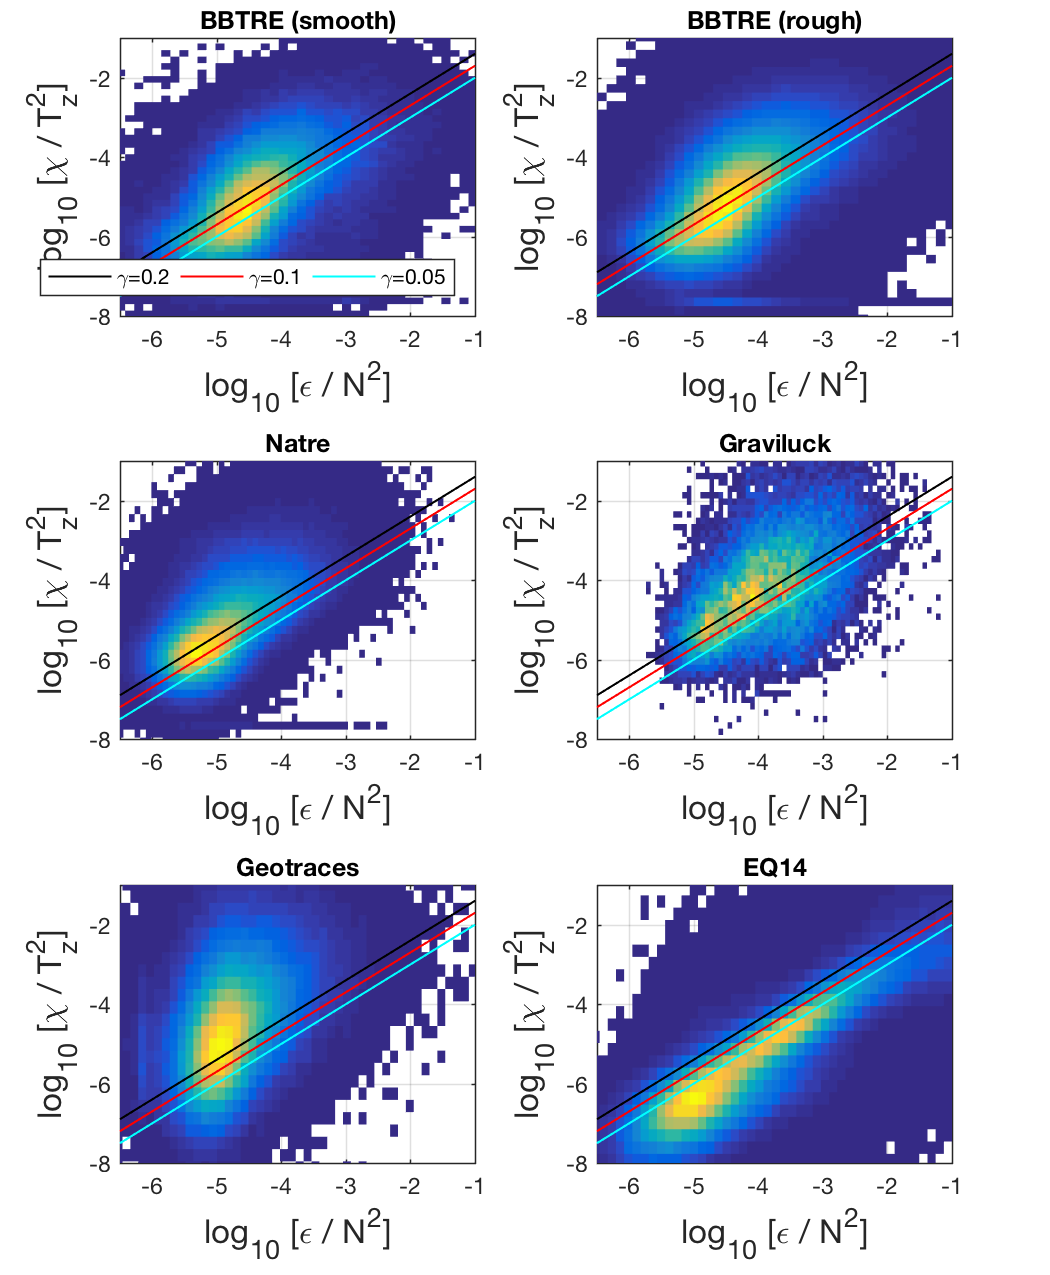
\includegraphics[scale=0.8]{chi_eps_norm_ALL.png}
\caption{$\chi$ vs $\epsilon$, normalized such that the slope is proportional to $\gamma$.}
\label{}
\end{figure}


\begin{figure}[htbp]
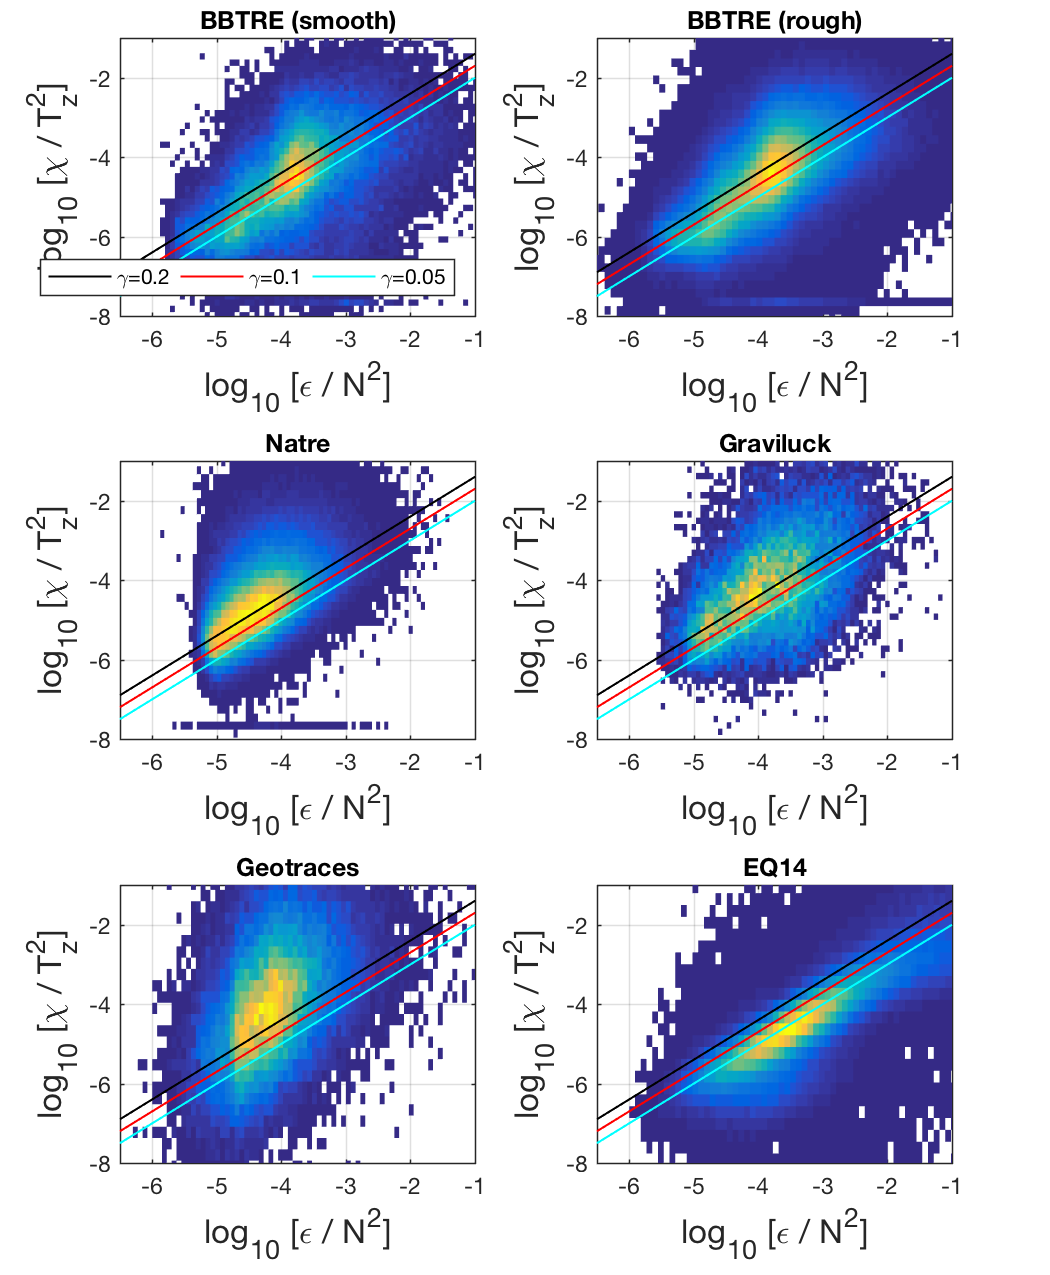
\includegraphics[scale=0.8]{chi_eps_norm_ALL_eps_thresh.png}
\caption{$\chi$ vs $\epsilon$, normalized such that the slope is proportional to $\gamma$. Values below estimated noise level of $log_{10}[\epsilon]=-10$ discarded.}
\label{}
\end{figure}








%~~~~~~~~~~~~~~~~~~~~~~~~~~~~~~~~~~~~~~~~~~~~~~~~~~
\end{document}  
%~~~~~~~~~~~~~~~~~~~~~~~~~~~~~~~~~~~~~~~~~~~~~~~~~~
%~~~~~~~~~~~~~~~~~~~~~~~~~~~~~~~~~~~~~~~~~~~~~~~~~~

